%~ \documentclass[letterpaper,times,draft]{sae}
\documentclass[letterpaper,times]{sae}

\usepackage[svgnames]{xcolor}
\definecolor{SAEblue}{RGB}{1,160,233}
\raggedright

\usepackage[justification=justified, singlelinecheck=false]{caption}  % ,figurename=Fig.,labelfont={it}
\DeclareCaptionFont{eightpt}{\fontsize{8pt}{11pt}\selectfont #1}
\captionsetup{font={eightpt,color=SAEblue}}

\usepackage{lineno}
\usepackage[utf8]{inputenc}

\usepackage{array}% http://ctan.org/pkg/array (also necessary for width calculations (for vert. lines)))
\newcolumntype{L}[1]{>{\raggedright\let\newline\\\arraybackslash\hspace{0pt}}p{#1}}
\newcolumntype{C}[1]{>{\centering\let\newline\\\arraybackslash\hspace{0pt}}p{#1}}
\newcolumntype{R}[1]{>{\raggedleft\let\newline\\\arraybackslash\hspace{0pt}}p{#1}}

\usepackage{graphicx}
\usepackage{multirow}
\usepackage{amsmath}

\newcommand{\ignore}[1]{}
\newcommand{\todo}[1]{\textcolor{red}{TODO: {#1}}}
\newcommand{\todr}[1]{\textcolor{purple}{CAN CUT: {#1}}}
\newcommand{\todm}[1]{\textcolor{green}{MOVE: {#1}}}
\newcommand{\case}[1]{\mbox{\textit{#1}}}
\newcommand{\textss}[1]{\textsuperscript{#1}}
\renewcommand{\deg}{$^\circ$}

\usepackage{nameref}
\usepackage{booktabs}

% Define "struts" as suggested by Claudio Beccari in
% a piece in TeX and TUG News, Vol. 2, 1993.
\newcommand\Tstrut{\rule{0pt}{4.6ex}}       % "top" strut
\newcommand\Bstrut{\rule[-0.9ex]{0pt}{0pt}} % "bottom" strut
\newcommand{\TBstrut}{\Tstrut\Bstrut} % top&bottom struts

%%% the following hides the section number while keeping their numbering for proper referencing in toc and \ref
\makeatletter
\def\@seccntformat#1{%
  \expandafter\csname c@#1\endcsname\c@section
  }
\makeatother

\usepackage{subfigure}
\usepackage{multimedia}

\DeclareMathOperator{\sign}{sign}
\newcommand{\quotes}[1]{``#1''}


\PaperTitle{2019-Updated \LaTeX\ document class for SAE Technical Papers}
\usepackage{calc} % to get proper table widths (subtracting colsep and black lines width

\makeatletter 
\renewcommand\@biblabel[1]{#1. } 
\makeatother

\AddAuthor{Louis Gagnon}{Department of Aerospace Science and Technology, Politecnico di Milano, Milano, Italy}
\PaperNumber{2019-XX-XXXX}
\SAECopyright{2019}



\begin{document}
\maketitle
\section{Abstract}
This \LaTeX\ class provides correct formatting according to the requirements
  for the publication of an SAE Technical Paper. It is supposed to be useful
  for authors publishing simulation models and similar containing lots of
  formulas. The style contains many features automating the formatting and
  thus, making it easier for the author to concentrate on contents. 

\section{Introduction}
\textbf{Important note: the author provides this updated template based on the original work of
Axel Franke (Lund Institute of Technology, Sweden).
The author is NOT affiliated with SAE International and does not guarantee
the accuracy of this template or the suggestions written therein.
This template is only a tentative to simplify the task of those who
wish to publish with SAE International and make use of \LaTeX\ typesetting software.}

This is a Level 1 heading, created with the command
\begin{verbatim}
\section{Introduction}
\end{verbatim}
As can be seen, the correct format (bold face and capitalized) is done by the
style -- the author does not need to care about that.

Here is a sample figure, namely Fig.~\ref{fig:sampleFigure}, followed by a sample table, namely, Table~\ref{tab:sampleTable}.
A simpler table without line returns and with a different number of columns to demonstrate the logic behind
the cell width calculation is shown in Table~\ref{tab:sampleTable2}. Finally,
a sample multifigure is shown, for whom wants to use subfigures, in Fig.~\ref{fig:sampleFigure2} and its subfigures
Figs.~\ref{fig:sampleFigure2A} to~\ref{fig:sampleFigure2C}.


\begin{figure}[!htb]
\centering
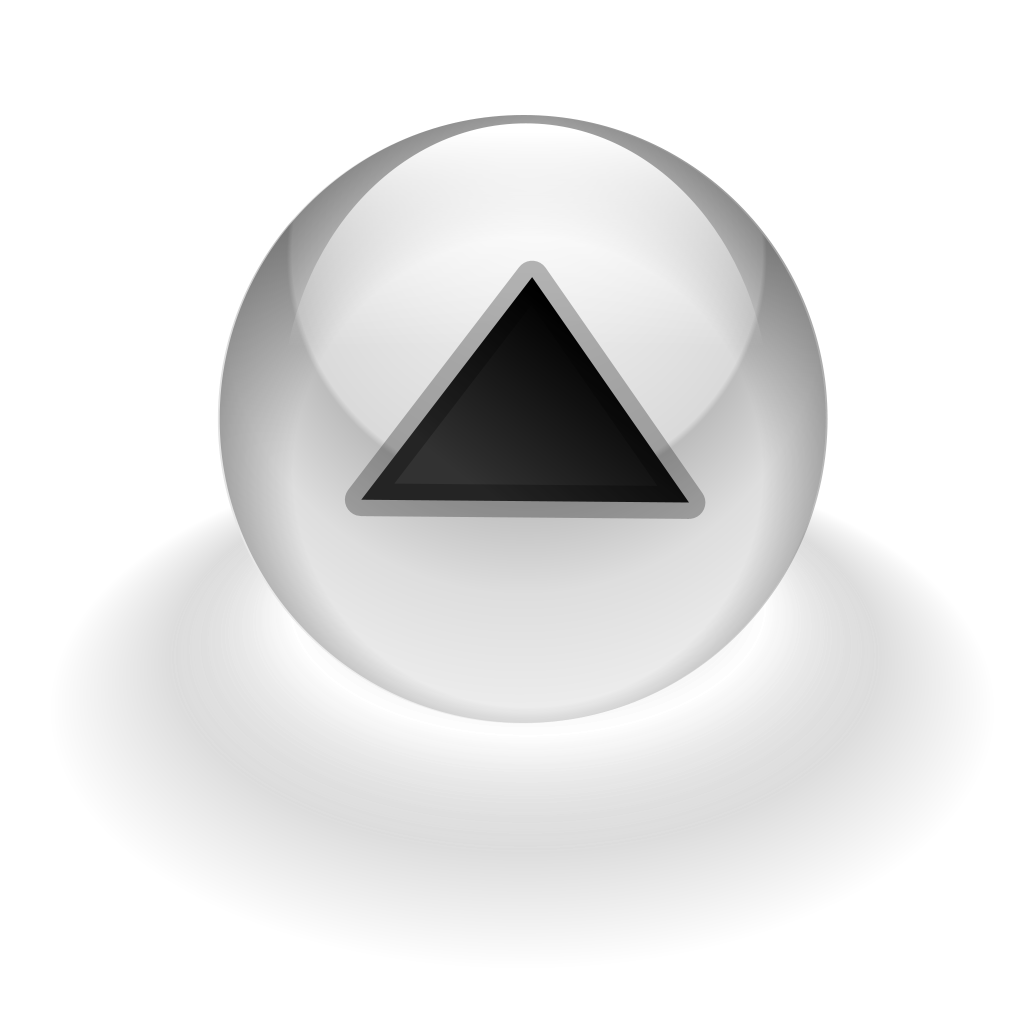
\includegraphics[width=0.3\textwidth]{sampleFigure}
\caption{Figure taken from wikimedia.org and openclipart.org.}
\label{fig:sampleFigure}
\end{figure}

\begin{table}[!htb]
\fontsize{8}{10}\selectfont
   \centering
   \caption{Example for a table.}\label{tab:sampleTable} 
   \begin{minipage}{\columnwidth}
\begin{tabular}{ |  L{0.8\linewidth-2\tabcolsep-1.3\arrayrulewidth} |  L{0.2\linewidth-2\tabcolsep-1.3\arrayrulewidth} | }
    \hline
a dimension & 0.009 m \\  \hline
another  & 0.24 m \\  \hline
a very long text describing another dimension to force a line return inside the table cell & 0.99 m \\  \hline
something that requires a footnote\footnote{An explanatory footnote.} & something \\  \hline
Writing an angle in degrees & 0$^{\circ}$ \\  \hline
  \end{tabular}\par
  \vspace{-0.15\skip\footins}
   \renewcommand{\footnoterule}{}
   \end{minipage}
\end{table}


\begin{table}[!htb]
\fontsize{8}{10}\selectfont
\centering
\caption{Some interesting results from our research.}\label{tab:sampleTable2}
\begin{tabular}{| L{0.1\columnwidth-2\tabcolsep-1.2\arrayrulewidth} | L{0.225\columnwidth-2\tabcolsep-1.2\arrayrulewidth} | L{0.225\columnwidth-2\tabcolsep-1.2\arrayrulewidth} | L{0.225\columnwidth-2\tabcolsep-1.2\arrayrulewidth} | L{0.225\columnwidth-2\tabcolsep-1.2\arrayrulewidth} |}
\hline
            & \textbf{Fx}         & \textbf{Fy}         & \textbf{T}          & \textbf{M}            \\ \hline
\textbf{A)}    & 0.453      & 1.00       & -       & -         \\  \hline
\textbf{B)} & 1.99       & 0.777      & 1.50       & -0.999       \\  \hline
	\end{tabular}
	\par
   \vspace{-0.15\skip\footins}
   \renewcommand{\footnoterule}{}
\end{table}


\begin{figure}[!htb]
\centering
\subfigure[Some info.]{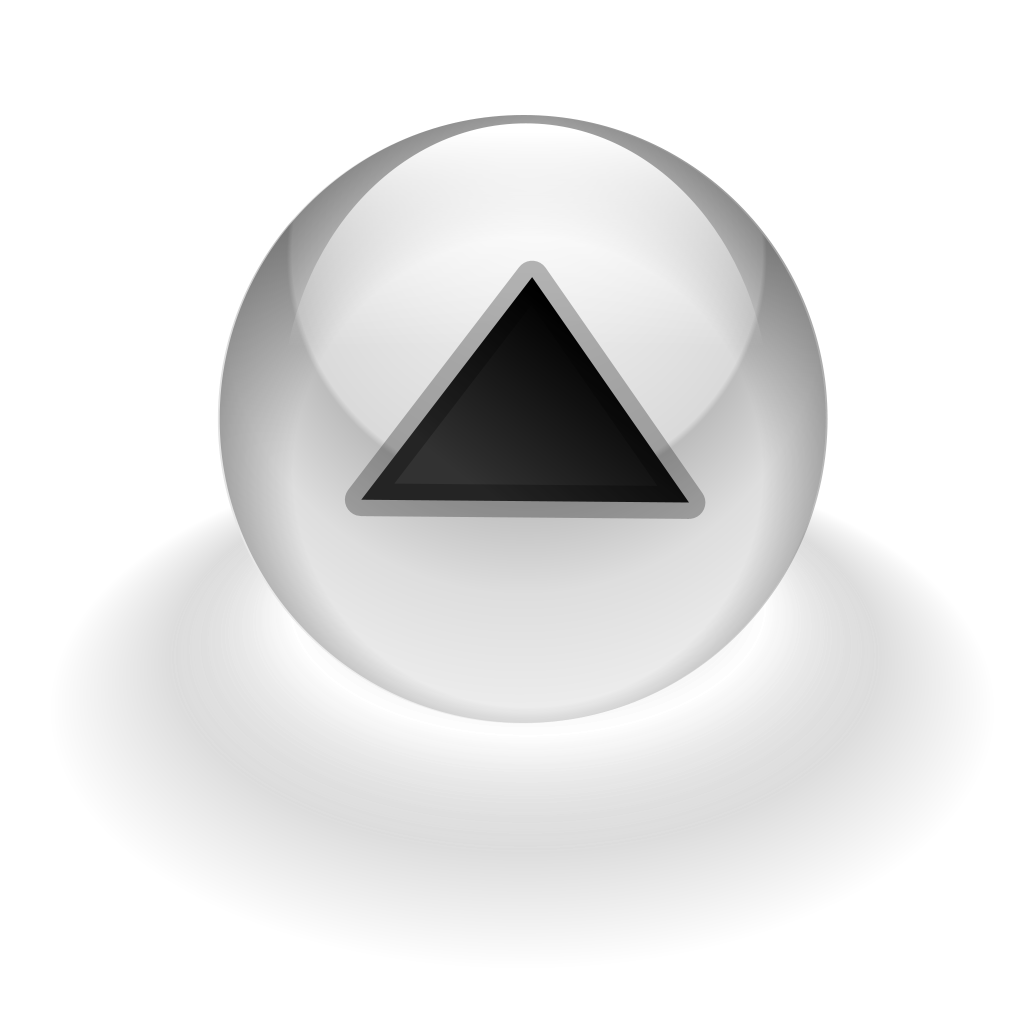
\includegraphics[height=.15\textheight]{sampleFigure}\label{fig:sampleFigure2A}}
\hspace{.01\textwidth}
\subfigure[Caption.]{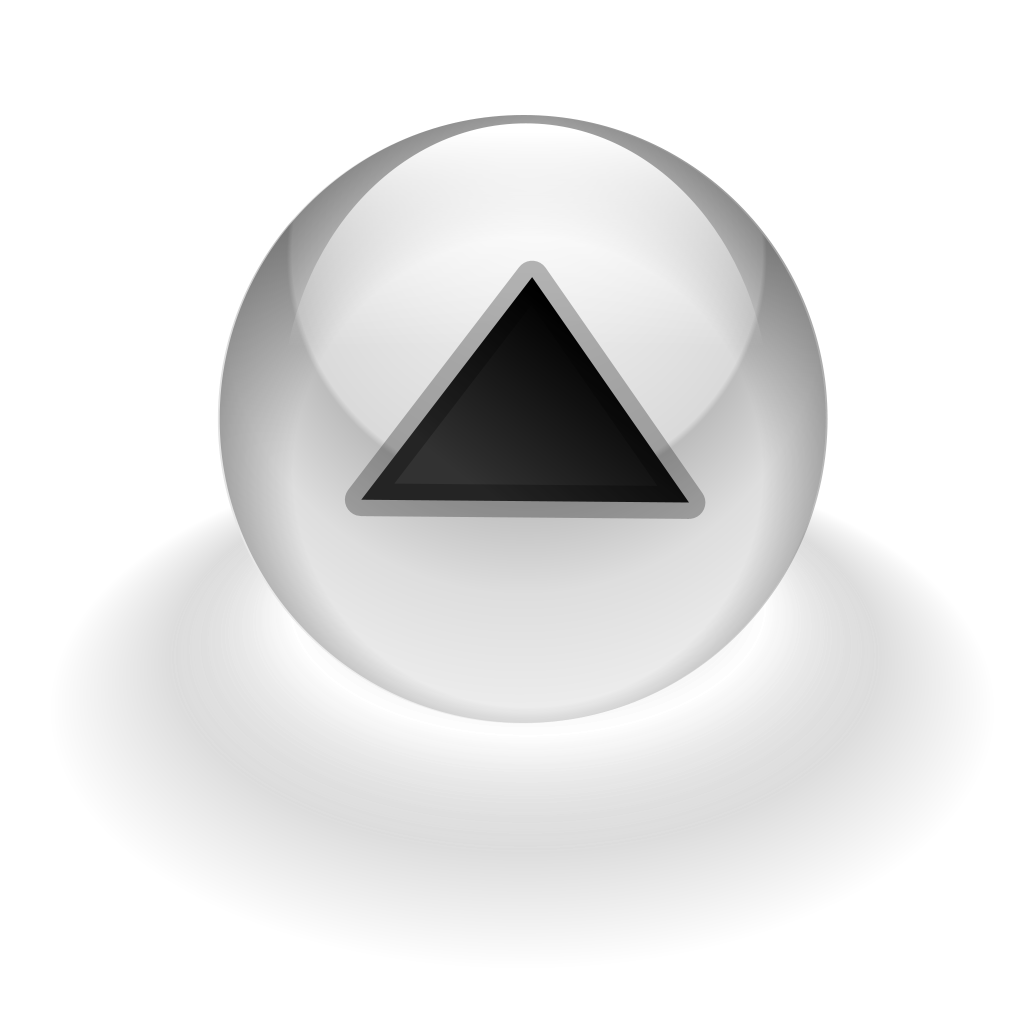
\includegraphics[height=.14\textheight]{sampleFigure}\label{fig:sampleFigure2B}}
\hspace{.01\textwidth}
\subfigure[More info.]{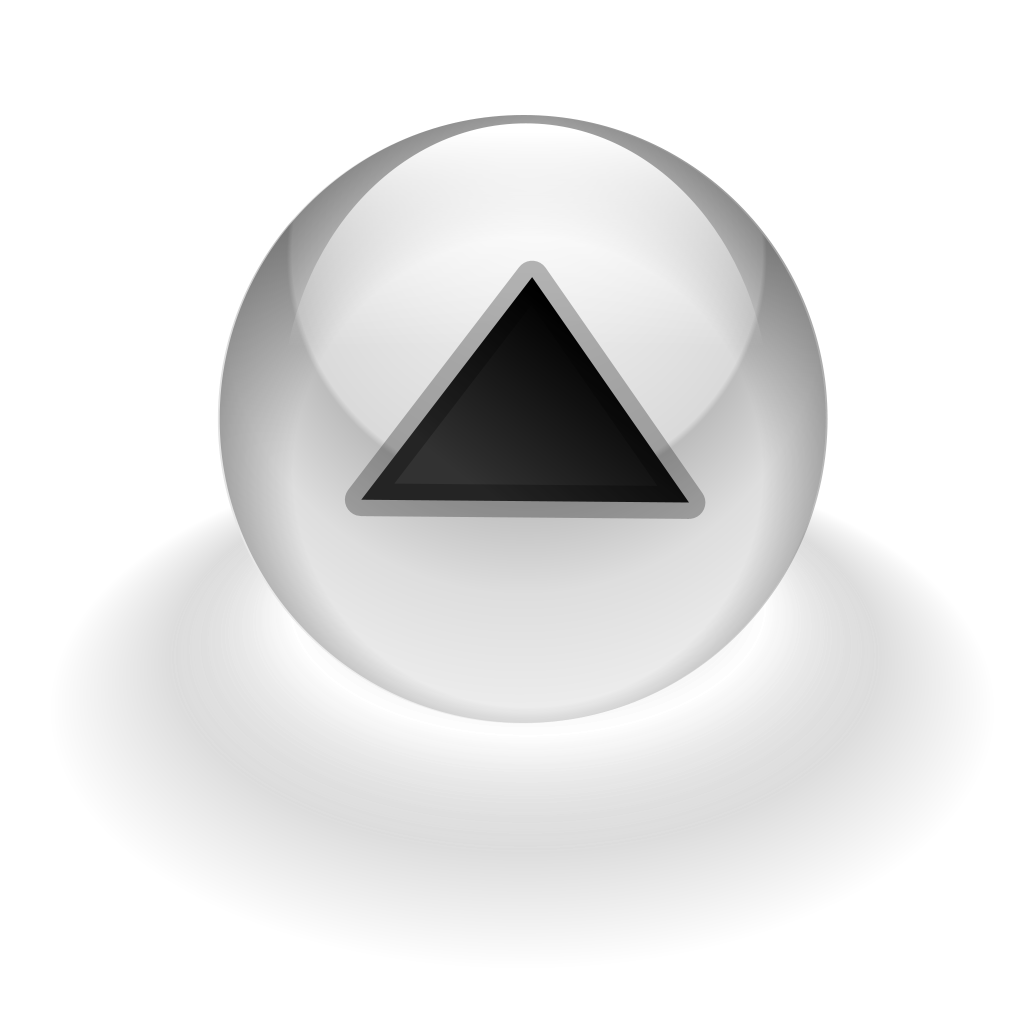
\includegraphics[height=.10\textheight]{sampleFigure}\label{fig:sampleFigure2C}}%
\caption{An overall caption for these figures.}
\label{fig:sampleFigure2}
\end{figure}

Some citations to interesting articles such as~\cite{GAGNON-OFW11-2016} or~\cite{gagAHS2014} can also be
added and then presented at the end of the document. These usually go after the conclusion or recommendation sections, respectively Sections~\ref{sec:concl} and~\ref{sec:recom}.



\section{Title and author information}
Title, author information, paper number and copyright are created in the
preface using the commands
\begin{verbatim}
\PaperTitle{Proposal for a \LaTeX\ document 
class for SAE Technical Papers}
\AddAuthor{Axel Franke}{Lund Institute of 
Technology, Sweden}
\PaperNumber{No number}
\SAECopyright{1999}
\end{verbatim}
Authors from the same affiliation should be added within one
\verb+\AddAuthor+ command. The general syntax is
\begin{verbatim}
\AddAuthor{Author1, Author2, ...}{Affiliation}
\end{verbatim}
The command may be used several times.


\subsection{A subheading}
This is a subheading which has been created as usual with the command
\begin{verbatim}
\subsection{A subsection}
\end{verbatim}
Also the following sub-subheading is formatted automatically by the style. 
\subsubsection{Subsubheading: general options of the style}
The \texttt{sae} \LaTeX\ style supports optional arguments which determine the
document font (Helvetica or Times) and the paper size (letterpaper or
A4). Default is Helvetica and A4. The letter format of this publication has
been obtained by the opening command
\begin{verbatim}
\documentclass[letterpaper]{sae}
\end{verbatim}
If Times is desired as document font, this can be achieved by using
\begin{verbatim}
\documentclass[letterpaper,times]{sae}
\end{verbatim}
or
\begin{verbatim}
\documentclass[times]{sae}
\end{verbatim}
The latter uses A4 as paper size. This concept has the advantage that document
font and the paper size can be changed easily at any time of the publication
process. 


\section{Conclusion}
\label{sec:concl}
Here can some interesting conclusion be presented.


\section{Recommendation}
\label{sec:recom}
Followed by a short recommendation based on the work done.


\bibliographystyle{ieeetr} % closest to SAE
\bibliography{sampleBib}

\section{Contact Information}
Louis Gagnon, Ph.D. \newline
Louis.Gagnon@Polimi.it

\section{Acknowledgments}
Some acknowledgments are always appreciated and sometimes compulsory! 

\section{Definitions, Acronyms, Abbreviations}

\begin{table}[h]
\centering
\begin{tabular}{L{0.1\textwidth} L{0.33\textwidth}}
\textbf{AMI} & Arbitrary Mesh Interface \\
\textbf{CFD} & Computational Fluid Dynamics \\
\textbf{RANS} & Reynolds-averaged Navier–Stokes \\
\end{tabular}
\end{table}


\onecolumn
\section{APPENDIX A}
\label{sec:figures}
This section can present figures that occupy too much space to include in the main text.
The authors can choose what should go in an appendix.
\clearpage


\section{APPENDIX B} %: Flow animations}
\label{sec:video}
\renewcommand{\thefigure}{B\arabic{figure}}
Sometimes a second appendix is necessary, for example, to give a link to some extra video material.


\end{document}
